\section{Análisis de Sistemas Tolerantes a Fallas en General}\label{sec:requerimentos_sistema_tolerancia_fallas}

%\section{Requerimientos de un Sistema con Tolerancia a Fallas}\label{sec:requerimentos_sistema_tolerancia_fallas}

% Primero se dan características de sistemas con redundancias de tiempo de tiempo real. De esto hay mucho en el libro de Kopetz y en su paper The Time Triggered Architecture. También en los papers que tengo impresos.

% Luego se menciona que esas características se hacen presente en varios de los trabajos de UAVs presentados en la sección anterior. Luego, explico los requerimientos como ya los tengo acá escritos.

% Volver a escribir la introducción a la sección
%A partir de los distintos casos presentados, en esta sección se busca relevar cuáles son las características comunes en sistemas con tolerancia a fallas. Se analizan las distintas alternativas y luego se mencionan los criterios tenidos en cuenta para el desarrollo de la computadora de vuelo. En este trabajo no se define a priori cuál es la arquitectura del sistema en cuanto al uso de redundancias, por lo que la computadora de vuelo debe tener cierta diversidad en cuanto a sus capacidades. 

El objetivo de esta sección es introducir el uso de redundancias como técnica para incrementar el nivel de seguridad en un sistema. Esta consiste en el uso de varias réplicas de distintos componentes, las cuales realizan las mismas tareas de manera independiente. En caso de que ocurra una falla, el sistema podrá seguir ejecutando su función de manera correcta, utilizando alguna de las demás réplicas. A partir de esto, se presentan las características de sistemas redundantes y los requerimientos que estos deben cumplir para funcionar adecuadamente. Finalmente, se muestra que si el sistema cumple con ciertas características, %en particular funcionar de manera sincronizada y utilizar un bus de comunicaciones, 
el funcionamiento del mecanismo para tolerar fallas puede simplificarse.

%Sistema de tiempo real, sincronización, uso de un bus de comunicaciones.

%Se explica la necesidad de la tolerancia a fallas como una medida para incrementar la seguridad de un sistema. 

%El objetivo de esta sección es presentar las características tenidas en cuenta para el sistema tolerante a fallas propuesto en este trabajo. 

%En esta sección se 

%Después presento el uso de redundancias como una técnica para la tolerancia a fallas. 

\subsection{Características de Sistemas Tolerantes a Fallas}

El objetivo del diseño tolerante a fallas consiste en mejorar la confiabilidad de un sistema, apuntando a que este pueda ejecutar su función correctamente, a pesar de la presencia de una cierta cantidad de fallas \cite{nelson1990fault}. Tal como lo indica su nombre, un sistema tolerante a fallas es aquel donde una falla no implica necesariamente un fracaso en el funcionamiento. Tampoco quiere decir que no ocurren fallas, sino que por el contrario, se acepta que las fallas pueden ocurrir. Lo que se busca es que el sistema igualmente pueda cumplir con su función de manera correcta.

%De esta última expresión se puede tomar una definición de lo que es un sistema tolerante a fallas.

% \begin{mydef}
%     \textbf{Sistema Tolerante a Fallas:} es aquel donde una falla no implica necesariamente un fracaso en el funcionamiento. Un sistema tolerante a fallas no es aquel donde no ocurren fallas, sino que más bien, se acepta que las fallas pueden ocurrir en el sistema, pero lo que se pretende es que el sistema pueda cumplir con su función de igual manera.
% \end{mydef}

De manera de introducir la nomenclatura que se encuentra en la bibliografía, se definen los siguientes términos:

\begin{itemize}
    \item Falla (\textit{Fault}): Es alguna condición anómala, no esperada.
    \item Error: Ocurre cuando una falla se manifiesta y produce un comportamiento fuera de lo esperado en alguna parte del sistema.
    \item Fracaso (\textit{Failure}): Quiere decir que el sistema no puede cumplir con su función de manera adecuada.
\end{itemize}

Por ejemplo en un UAV, la información proveniente de los distintos sensores se utiliza para estimar la pose del vehículo. Si un sensor entrega información que no se corresponde con la realidad, luego esto implicará a una \textbf{falla}. Si esta no es detectada y corregida, luego la computadora de vuelo utilizará esta información para realizar los cálculos de estimación, obteniendo una estimación incorrecta de la pose. Esto representa un \textbf{error}. Finalmente, esto causará que tampoco pueda seguir su trayectoria correctamente, lo que implicará un \textbf{fracaso} del sistema.

Se define la confiabilidad de un sistema como la probabilidad de que este pueda cumplir con su función de manera correcta en un intervalo de tiempo $[t_0;t]$, dado que en el instante inicial $t_0$ podía hacerlo \cite[p.~10]{kopetz-2011}:

\begin{equation}
    R(t) = \mathtt{P}\left( \text{funcionamiento correcto en $t$} | \text{funcionamiento correcto en $t_0$} \right)
    \label{eq:Reliability}
\end{equation}

En el caso en el que se tuviera un sistema sin ningún mecanismo de tolerancia, la ocurrencia de una falla implicaría un funcionamiento incorrecto, es decir un fracaso. Esto quiere decir que la confiabilidad sería exactamente igual a la probabilidad de que no ocurra ninguna falla en el intervalo $[t_0;t]$ \cite{nelson1990fault}. En este caso, la confiabilidad podría expresarse como en la ecuación \eqref{eq:Reliability_3} y la única manera de mejorarla sería incrementando la probabilidad de que no ocurra ninguna falla en el intervalo $[t_0;t]$.

\begin{equation}
    R(t) = \mathtt{P}\left( \text{no ocurrio ninguna falla en $[t_0;t]$} \right)
    \label{eq:Reliability_3}
\end{equation}

Si es posible demostrar que el sistema cumple con un determinado requerimiento de confiabilidad, luego no sería necesario el uso de técnicas de tolerancia a fallas. La manera de hacer esto puede ser por ejemplo, utilizando componentes o módulos de muy buena calidad lo suficientemente confiables \cite{nelson1990fault}. Sin embargo, esto puede ser muy costoso, pensando en que un sistema puede estar compuesto de muchos componentes y cada uno de ellos puede manifestar una gran cantidad de posibles fallas. Sumado a esto, se dificulta la etapa de diseño de un sistema, ya que cualquier error que no se haya tenido en cuenta puede llegar a causar una falla y por ende un fracaso del sistema.

El uso de técnicas para tolerar fallas representa una actitud más conservadora, ya que se acepta que las fallas pueden ocurrir. Dado que en el intervalo $[t_0;t]$ puede o no ocurrir una falla, la probabilidad de que el sistema pueda cumplir su función en $t$ puede expresarse como en la ecuación \eqref{eq:Reliability_2}. Si no ocurre ninguna falla, luego el sistema podrá seguir cumpliendo su función en $t$. Además, si llegase a ocurrir una falla, pero el sistema tiene la capacidad de tolerarla, luego el sistema de igual manera podrá seguir cumpliendo su función en el instante $t$.

\begin{equation}
    \begin{aligned}
        R(t) &= \mathtt{P}\left( \text{no ocurrio una falla en $[t_0;t]$} \right)\\ &+ \mathtt{P}\left( \text{funcionamiento correcto en $t$}|\text{ocurrió una falla en $[t_0;t]$} \right) \ \mathtt{P}\left( \text{ocurrió una falla en $[t_0;t]$} \right)
    \end{aligned}
    \label{eq:Reliability_2}
\end{equation}

La probabilidad de que el sistema funcione correctamente a pesar de la falla, está pesada por la probabilidad de ocurrencia de dicha falla. A partir de esto se desprende que aplicar técnicas de tolerancia a fallas para cada una de las posibles fallas puede resultar exhaustivo, principalmente porque deberían conocerse todas las fallas posibles. Lo que se propone es considerar solo aquellas fallas cuya criticidad es alta. Una de estas correspone al ejemplo antes mencionado, donde una falla de un sensor puede causar el fracaso de la misión del vehículo.

%A modo de ejemplo, una \textbf{falla en un sensor de la computadora de vuelo puede generar una lectura incorrecta}. En consecuencia, esto decantará en un \textbf{error, es decir, en un cálculo de la ley de control incorrecto}. Finalmente, este error puede llevar al \textbf{fracaso de la misión, por ejemplo si el vehículo no es capaz de seguir una trayectoria dada en tiempo y forma}. Esto da a entender que una falla en un sensor es crítica y que por ende requiere la aplicación de técnicas de tolerancia a fallas.

%Aquí se habla de falla en un sensor como algo general. Un sensor podría fallar de muchas maneras y debido a muchas razones. Por ejemplo, puede dejar de funcionar por un defecto propio del componente, puede entregar lecturas erróneas debido a interferencias electromagnéticas, por efectos de la temperatura, falta de calibración, etc. Cada uno de estos requeriría la aplicación de un mecanismo tolerante a fallas.

%Teniendo en consideración las consecuencias que puede traer el fracaso del sistema en cuestión, resulta adecuado tomar una actitud conservadora y adoptar técnicas de tolerancia a fallas, aceptando que estas pueden ocurrir.

\subsection{Uso de Redundancias}

%Todos los trabajos y ejemplos presentados en la sección \ref{sec:estado_del_arte} comparten la característica de implementar la tolerancia a fallas utilizando varias copias del mismo elemento de hardware. Estas copias trabajan en paralelo y se comparan los resultados obtenidos por cada una de ellas. Las fallas se detectan cuando ocurre una diferencia en los resultados de las copias. Esta es la principal técnica de tolerancia a fallas \cite{nelson1990fault}\cite{prasad1989fault}\cite{lala1994architectural}\cite{kopetz2003time} y es la que se utilizará en este trabajo. Esto quiere decir, que se replica el hardware en el sistema y cada réplica realiza la misma tarea en paralelo. De esta forma, si una de las réplicas presenta una falla (arbitraria por ejemplo), esta puede detectarse a partir de la comparación con las demás réplicas, o incluso pasar desapercibida. Utilizando la nomenclatura definida en la sección \ref{subsec:introduccion_al_analisis_de_tolerancia_a_fallas}, que una falla pase desapercibida quiere decir que no se manifiesta como un error, sino que esta es contenida. A continuación se presentan algunas arquitecturas redundantes para la tolerancia a fallas.

La detección de una falla en el sistema puede llevarse a cabo de distintas formas. Volviendo sobre el ejemplo antes presentado de la estimación de la pose del vehículo, una forma de detectar la falla podría ser analizando si el valor que entrega el sensor ``tiene sentido''. Para esto último sería necesario definir un algoritmo que pueda discriminar entre un valor entregado por el sensor que ``tiene sentido'' y uno que no. Una forma muy simple podría ser monitoreando que los valores entregados por el sensor se encuentren dentro de cierto rango. Esto sería para el caso de un sensor, aunque se requeriría un mecanismo similar para los demás sensores u otros componentes del sistema.

En un sistema de tiempo real, como lo es el control de vuelo de un vehículo, la computadora de vuelo debe aplicar una nueva acción sobre sus actuadores de manera periódica. Esto impone una restricción en el tiempo de ejecución sobre los algoritmos que detecten las posibles fallas, ya que no deben perjudicar la periodicidad del sistema de control del vehículo.

A su vez, podría ocurrir que la información de los sensores sea correcta, pero que el cálculo de la estimación de la pose o de la ley de control presente un resultado incorrecto. Para tolerar esto, se requerirían otros algoritmos para la detección de estos errores, los cuales también deben tener un tiempo de ejecución que no perjudique la periodicidad del sistema de control del vehíuclo.
%En caso de que ocurra una falla el mecanismo de detección de fallas implique un algoritmo con un procesamiento, donde por ejemplo se contemple un caso donde el sensor no entregue ningún valor. 

Otra forma de detectar fallas y errores puede ser a partir del uso de redundancias. %Esta es la principal técnica de tolerancia a fallas \cite{lala1994architectural}. 
Tanto las fallas como los errores pueden detectarse a partir de la comparación de resultados entre réplicas. Esto implica una carga computacional mucho menor, ya que basta con comparar los resultados entre réplicas para detectar las fallas que puedan ocurrir. 
%Esta técnica plantea que, tanto las fallas como los errores pueden detectarse a partir de la comparación de resultados, contra una referencia la cual es considerada correcta. Esto implica una carga computacional mucho menor, ya que no se requieren algoritmos demasiado complejos para detectar las fallas, ya que para esto basta con comparar el resultado obtenido con el resultado de referencia.
%Este valor de referencia que se asume correcto, se obtiene a partir del uso de varias réplicas de hardware en el sistema. 
Por ejemplo, podría utilizarse más de un sensor del mismo tipo para tolerar fallas de sensores, o más de una computadora de vuelo, para tolerar errores en los cálculos de la ley de control y en los sistemas de navegación.

Todos los trabajos presentados en la sección \ref{sec:estado_del_arte} comparten la característica de implementar la tolerancia a fallas utilizando varias réplicas del mismo elemento de hardware. A partir de estos se pudo ver que existen muchas configuraciones típicas, algunos utilizan 2 réplicas, otros 3 o incluso 4. Con el objetivo de entender las capacidades de cada una de estas, a continuación se analizan las distintas configuraciones.

\subsubsection{Redundancia Doble}

Una configuración muy simple es la redundancia doble. En este tipo de sistemas se utilizan 2 réplicas las cuales trabajan en paralelo ejecutando las mismas tareas y comparando sus resultados entre sí. La ocurrencia de una falla se detecta cuando ocurre una discrepancia entre los resultados obtenidos por cada una de las réplicas.

\begin{figure}[htb]
    \centering
    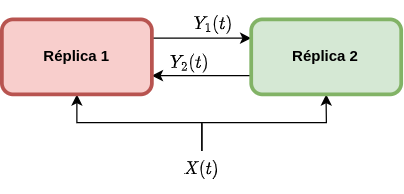
\includegraphics[width=0.5\textwidth]{img/redundancia_doble.png}
    \caption{Esquema de redundancia doble. La entrada $X(t)$ es utilizada por ambas réplicas y cada una de ellas obtiene una salida $Y_1(t)$ e $Y_2(t)$. Si ocurre que $Y_1(t) \neq Y_2(t)$, luego esto implicará una falla de alguna de las réplicas. }
    \label{fig:redundancia_doble}
\end{figure}

% \begin{figure}[htb]
%     \centering
%     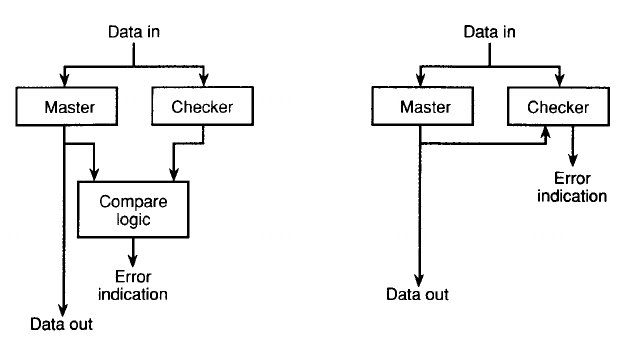
\includegraphics[width=0.6\textwidth]{img/3_4_lockstep_architecture.png}
%     \caption{En la figura de la izquierda, dos sistemas ejecutan las mismas operaciones, mientras que otro sistema externo se encarga de comparar las salidas de ambos para detectar errores. En la figura de la derecha, el bloque comparador se encuentra integrado en el sistema \textit{checker}. La imagen fue extraida de \cite{nelson1990fault}.}
%     \label{fig:3_4_lockstep_architecture}
% \end{figure}

Si bien este tipo de arquitectura permite detectar fallas a partir de la comparación de resultados, no es posible identificar cuál de las réplicas fue la que falló. Para lograr esto último, cada una de estas debería ejecutar una rutina para detectar si ellas fueron las que cometieron el error o no \cite{baleani2003fault}. En un sistema de tiempo real, donde existe un requerimiento temporal para obtener un nuevo resultado de la estimación de la pose y de la acción de control sobre los motores, no resulta aceptable que el sistema deba detenerse o retrasar su ejecución para realizar este análisis en pleno vuelo. Debido a esto es que esta configuración no se presta para ser utilizada en sistemas de tiempo real como el de la computadora de vuelo.

%ya que la rutina de ejecución para la detección de la falla perjudica el requerimiento temporal propio de este tipo de sistemas. No resulta adecuado que el sistema de control de vuelo del vehículo tenga que suspenderse hasta que se pueda detectar cuál de las dos réplicas fue la que presentó la falla.

%En la figura \ref{fig:3_4_lockstep_architecture} se muestran dos configuraciones. La configuración de la derecha puede ser implementada a través de dos CPUs totalmente independientes (a veces denominada \textit{Loosely-Synchronized Dual Processor Architecture}) o a través del uso de un procesador de dos núcleos, donde uno sería el \textit{Master} y otro el \textit{checker}\cite{baleani2003fault}. En esta última, ambos se encuentran sincronizados por estar en el mismo chip y compartir fuente de clock. En la figura \ref{fig:3_4_lockstep_architecture_2} se muestra un esquema de ambos casos.

% \begin{figure}[htb]
%     \centering
%     \begin{subfigure}[b]{0.49\textwidth}
%         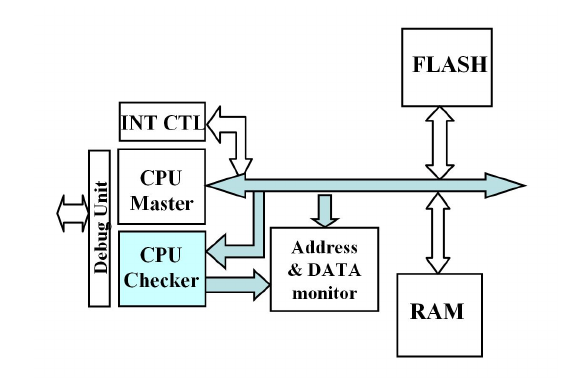
\includegraphics[width=\textwidth]{3_4_lockstep_dual_core.png}
%         \caption{Lockstep dual processor architecture.}
%         \label{fig:3_4_lockstep_dual_core}
%     \end{subfigure}
%     \begin{subfigure}[b]{0.49\textwidth}
%         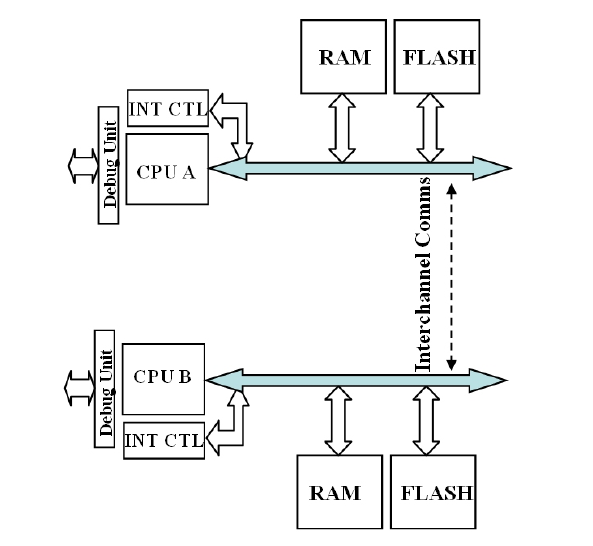
\includegraphics[width=\textwidth]{3_4_loosely_synchronized_dual_processor_architecture.png}
%         \caption{Loosely synchronized dual processor architecture.}
%         \label{fig:3_4_loosely_synchronized_dual_processor_architecture}
%     \end{subfigure}
%     \caption{Se muestran dos casos para un sistema con redundancia doble. La imagen fue extraida de \cite{baleani2003fault}.}
%     \label{fig:3_4_lockstep_architecture_2}
% \end{figure}

%Debido a que no se puede saber cuál de las dos CPUs cometió el error, esta arquitectura plantea que en el caso en el que la comparación entre ambas CPUs genere una discrepancia en los resultados, cada una de ellas deben ejecutar un algoritmo interno, para detectar si ellas fueron las que cometieron el error o no. En \cite{zhang2015dual} y en \cite{SolanoPerez2019} se pueden encontrar proyectos de redundancia doble para UAVs.

\subsubsection{Redundancia Triple}

Esta arquitectura puede encontrarse en la literatura con el nombre \textit{Triple Modular Redundancy (TMR)} \cite{lyons1962use} y consiste en el uso de 3 réplicas, las cuales computan los mismos resultados en paralelo. En esta configuración se asume que solamente 1 de las 3 réplicas presentará una falla a la vez. A diferencia de la redundancia doble, en esta configuración sí es posible detectar cuál de las réplicas fue la que presentó la falla a partir de la comparación de resultados, ya que solamente 1 de los resultados será distinto a los otros 2.

\begin{figure}[htb]
    \centering
    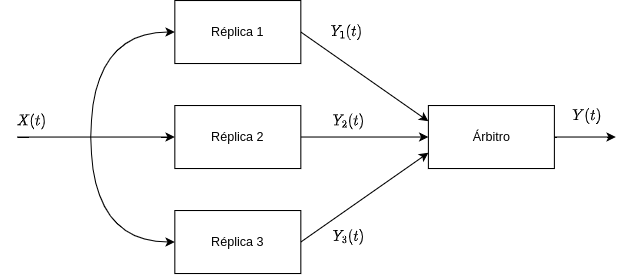
\includegraphics[width=0.7\textwidth]{TMR.png}
    \caption{Esquema de redundancia triple. La entrada $X(t)$ es utilizada por las 3 réplicas para obtener sus respectivos resultados $Y_1(t)$, $Y_2(t)$ e $Y_3(t)$. Un bloque denominado árbitro se encarga de seleccionar el valor correcto para la salida $Y(t)$.}
    \label{fig:TMR}
\end{figure}

%Esto resulta especialmente útil en sistemas de tiempo real, donde no puede detenerse el sistema para realizar una verificación interna. Esto se denomina \textit{Fault Masking}.

%En dicho caso, los resultados de dos computadoras serán iguales y la de la tercera será distinto, por lo que solamente se descarta el resultado erróneo. En la figura \ref{fig:3_5_TMR} se muestra un diagrama con la arquitectura TMR. Una diferencia de esta arquitectura respecto de la doble redundancia, es el hecho de que puede detectarse cuál de las computadoras falló y además, no es necesario que todas las computadoras ejecuten una rutina para verificar si cometieron el error o no. Esto resulta especialmente útil en sistemas de tiempo real, donde no puede detenerse el sistema para realizar una verificación interna. Esto se denomina \textit{Fault Masking}.

Como se muestra en la figura \ref{fig:TMR}, además de las 3 réplicas se utiliza un elemento adicional denominado árbitro. Este tiene la tarea de comparar los resultados de las 3 réplicas y determinar cuál es el resultado correcto. De esta manera no solo es posible detectar cuál de las réplicas fue la que falló, sino que además es posible obtener una salida correcta $Y(t)$, sin la necesidad de que el sistema deba deternse a hacer un análisis, algo que sí ocurría en la redundancia doble. Esto resulta especialmente útil en sistemas de tiempo real, donde continuamente debe proveerse una nueva salida del sistema de navegación y de la actuación de los motores. Esto se denomina enmascaramiento de la falla \cite{nelson1990fault}, ya que la falla de una de las réplicas queda cubierta por el valor correcto entregado por las otras 2. Debido a que la selección de la salida correcta $Y(t)$ se ejecuta a través de una votación entre los valores $Y_1(t)$, $Y_2(t)$ e $Y_3(t)$, este bloque también es llamado voter en inglés \cite{lyons1962use}.

El hecho de que el árbitro sea el que determine cuál es el resultado correcto, necesariamente implica que este debe ofrecer una confiabilidad, $R(t)$, mucho mayor que la de cada una de las 3 réplicas. Esto se denomina punto singular de falla, ya que una falla en el árbitro inevitablemente genera un fracaso de todo el sistema. Típicamente el árbitro se constituye por hardware más robusto, volviéndolo más costoso. Por ejemplo, cada réplica puede contener un procesador como un microcontrolador COTS, mientras que el árbitro puede estar implementado con un ASIC específico para esa aplicación \cite{hiergeist2017internal}.

% \begin{mydef}
%     \textbf{Single-Point Failure}: si la arquitectura del sistema es tal que una parte del sistema X fracasa en cumplir su trabajo dentro del sistema, luego el sistema completo fracasará en cumplir su función. En dicho caso, X es un punto único de falla.
% \end{mydef}

Para eliminar este punto singular de falla, sería necesario utilizar varias réplicas del árbitro \cite{nelson1990fault}\cite{lyons1962use}, lo que permitiría enmascarar errores que estos puedan cometer. A priori esto podría parecer inviable, ya que se requeriría una gran cantidad de componentes, 3 computadoras de vuelo + 3 bloques árbitro, solo para poder tolerar la falla de 1 de los componentes. Además, teniendo en cuenta el argumento de que los árbitros generalmente son más costosos que las réplicas individuales, se encarecería mucho el sistema completo.

%Una forma de eliminar el punto singular de falla consiste es utilizar varias réplicas del árbitro \cite{nelson1990fault}\cite{lyons1962use}, lo que permitiría enmascarar errores que estos puedan cometer. La arquitectura sería como la que se muestra en la figura \ref{fig:TMR_triple_arbitro}. Esta arquitectura es más compleja que las anteriores, ya que se requiere una gran cantidad de componentes, 3 computadoras de vuelo + 3 bloques árbitro, dando un total de 6. Además, pensando en que se argumentó que los aárbitros generalmente son más costosos que las réplicas individuales, esto encarecería mucho al sistema completo.

% \begin{figure}[htb]
%     \centering
%     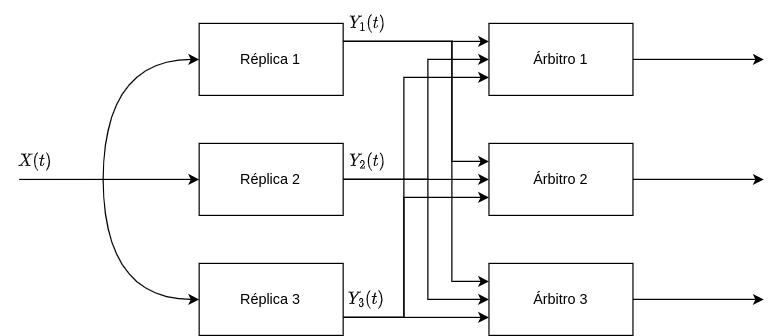
\includegraphics[width=0.7\textwidth]{img/TMR_triple_arbitro.png}
%     \caption{Arquitectura TMR con redundancia del árbitro.}
%     \label{fig:TMR_triple_arbitro}
% \end{figure}

%Los tres elementos \textit{Voter} reciben las mismas entradas y en el caso de que ninguno de los \textit{voters} cometa un error, dado que las entradas de los \textit{Voters} son exactamente iguales, luego los tres decidirán por el mismo resultado como el valor correcto.

%Esta arquitectura es más compleja que las anteriores, ya que requiere una gran cantidad de nodos, 3 FCCs + 3 bloques votantes, dando un total de 6. Además, pensando en que se argumentó que los votantes generalmente son más confiables que las FCCs, la triplicación del bloque \textit{Voter} encarece mucho al UAV.

%Otra cuestión que aparece en esta arquitectura, es que si bien los votantes generan cada uno un valor de salida, al fin y al cabo será uno solo el valor a utilizar. En la figura \ref{fig:3_3_2_consenso_1}, cada voter tiene su propia salida, pero en algún punto se deberá decidir cuál de las tres salidas es la que se va a utilizar como correcta. Por ejemplo, si el valor de salida es la señal de actuación de un motor, luego los tres resultados del voter deberan enviarse a algún modulo encargado de controlar dicho motor.

Una alternativa podría ser que las mismas réplicas sean las que ejecuten la votación, comparando sus salidas con las de sus pares. Esto es algo que se lleva a cabo en uno de los trabajos presentados en la sección \ref{sec:estado_del_arte}, donde los autores presentan resultados para una arquitectura con redundancia cuádruple, donde los mismos microcontroladores de cada réplica son los encargados de realizar la votación. %\cite{hiergeist2018implementation}.
%Como medida para evitar esto último, los bloques votantes pueden integrarse dentro de cada una de las FCC. Esto quiere decir, que en lugar de tener 3 bloques votantes, las mismas FCC sean las encargadas de realizar la votación. 
%En el artículo \cite{hiergeist2017internal} se propone que los microcontroladores automotivos ofrecen las interfaces necesarias para implementar una red redundante para tolerar fallas. 
%En el artículo \cite{hiergeist2018implementation}, los mismos autores presentan resultados para una arquitectura con redundancia cuádruple, donde los mismos microcontroladores de cada FCC son los encargados de realizar la votación. 
Para el caso de una arquitectura de redundancia triple, puede diagramarse como en la figura \ref{fig:TMR_sin_arbitro}.

% \begin{figure}[htb]
%     \centering
%     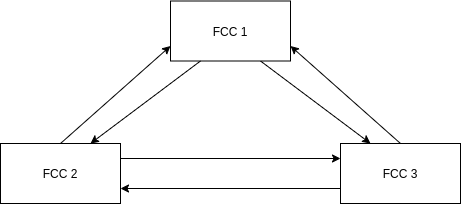
\includegraphics[width=0.5\textwidth]{img/3_5_TMR_2.png}
%     \caption{Arquitectura de redundancia trple, donde los bloques votantes son las mismas FCCs. Los votantes se encuentran integrados dentro de cada FCC.}
%     \label{fig:3_5_TMR_2}
% \end{figure}

\begin{figure}[htb]
    \centering
    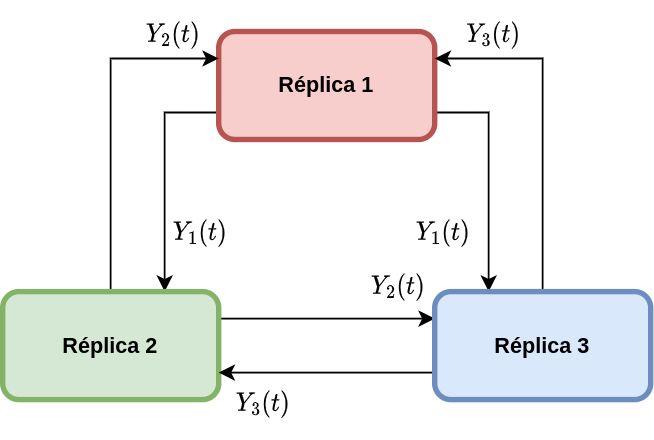
\includegraphics[width=0.5\textwidth]{img/TMR_sin_arbitro.png}
    \caption{Cada una de las réplicas comparte los resultados con sus pares. Luego, cada una de ellas realiza una votación sobre los valores para obtener el resultado correcto y detectar fallas.}
    \label{fig:TMR_sin_arbitro}
\end{figure}

Puede encontrarse bibliografía en la que esta configuración, donde cada réplica contiene su propio elemento voter, se define como una característica fundamental de la \textit{Triple Modular Redundancy (TMR)} \cite[p.~156]{kopetz-2011}. Sin embargo, hay otros requerimientos que deben cumplirse para que el sistema funcione de manera exitosa. Uno de ellos es la necesidad de la sincronización entre réplicas, la cual se explica a continuación.

\subsubsection{Necesidad del Sincronismo entre Réplicas}\label{sec:necesidad_del_sincronismo}
%\subsubsection{Sincronismo de los Nodos}
%\subsection{Sincronismo de los Nodos}

Las tareas de estimación de la pose del vehículo, y de cálculo de la acción de control a aplicar sobre los motores comprenden tareas con requerimientos temporales, ya que periódicamente debe obtenerse un nuevo valor, acorde al estado en el que se encuentra el vehículo. En la figura \ref{fig:evolucion_estados_real_time} se muestra un ejemplo donde $Y(t)$ corresponde a la estimación de la pose del vehículo. El valor de este resultado solo tiene validez durante el intervalo de tiempo $[t;t+1)$. Lo mismo ocurre con todos los siguientes resultados $Y(t+N)$, los cuales solamente serán válidos durante los intervalos $[t+N;t+N+1)$.

%La computadora de vuelo comprende un sistema de tiempo real. Los resultados que se obtienen son sobre variables que tienen validez solamente durante un breve período de tiempo. Esto ocurre tanto para la estimación de la pose del vehículo, como para la acción de control a aplicar sobre los motores. En la figura \ref{fig:evolucion_estados_real_time} se presenta un ejemplo donde $Y(t)$ corresponde a una estimación de la pose del vehículo. El valor de este resultado solo tiene validez durante el intervalo de tiempo $[t;t+1)$. Lo mismo ocurre con todos los siguientes resultados $Y(t+N)$, los cuales solamente serán válidos durante los intervalos $[t+N;t+N+1)$. Cada una de las réplicas del sistema continuamente calcula estos resultados $Y(t)$, $Y(t+1)$, etc, de manera periódica.

%Prácticamente en todos los trabajos que se presentaron en la sección \ref{sec:estado_del_arte} se menciona que las réplicas trabajan de manera sincronizada. Esta necesidad surge debido a que la computadora de vuelo comprende un sistema de tiempo real. Todos los resultados que se obtienen son sobre variables que tienen validez solamente durante un período de tiempo. Esto se representa en la figura \ref{fig:evolucion_estados_real_time}, donde el resultado $Y(t)$ solo es válido durante el intervalo de tiempo $[t;t+1)$. Lo mismo ocurre con todos los resultados $Y(t+N)$, los cuales solamente serán válidos durante los intervalos $[t+N;t+N+1)$. Cada una de las réplicas del sistema continuamente calcula estos resultados $Y(t)$, $Y(t+1)$, etc, de manera periódica.

\begin{figure}[htb]
    \centering
    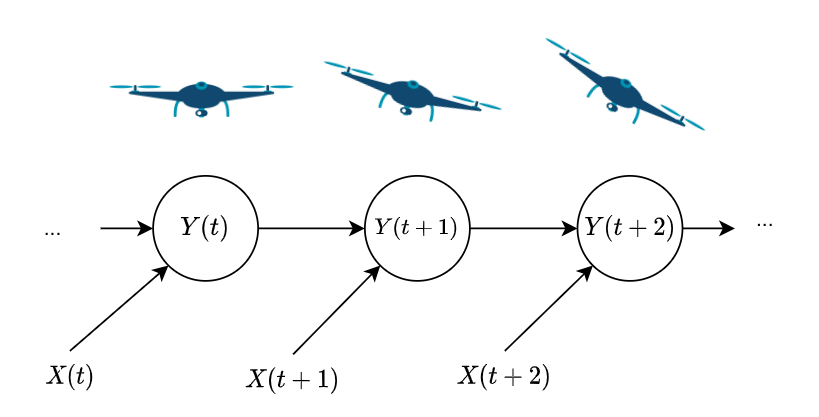
\includegraphics[width=0.8\textwidth]{img/evolucion_estados_real_time.png}
    \caption{En cada instante de tiempo $t$, $t+1$ y $t+2$ el vehículo se encuentra en un estado distinto, por lo que el algoritmo de estimación de la pose generará 3 resultados diferentes $Y(t)$, $Y(t+1)$ e $Y(t+2)$. Las entradas $X(t)$, $X(t+1)$ y $X(t+2)$ corresponden a mediciones de los distintos sensores.}
    \label{fig:evolucion_estados_real_time}
\end{figure}

Al utilizar varias réplicas de la computadora de vuelo, cada una de estas continuamente calcula estos resultados $Y(t)$, $Y(t+1)$, etc, de manera periódica. Luego, a partir de las comparaciones es que se detectan y se enamscaran las fallas. Para que estas comparaciones tengan sentido, deben llevarse a cabo sobre resultados que se correspondan temporalmente. Esto implica que todas las réplicas deben calcular sus correspondientes resultados $Y_i(t)$ al mismo tiempo.

Cada una de las réplicas ejecuta una serie de tareas para realizar cálculos sobre la estimación de la pose y sobre la acción de control. La manera de asgurar que estas se ejecuten al mismo tiempo es a través de un mecanismo de sincronización. Esto es lo que sucede prácticamente en todos los trabajos que se presentaron en la sección \ref{sec:estado_del_arte} para UAVs.

En la práctica una sincronización perfecta sería algo excesivo. Sin embargo esto no es necesario y puede tolerarse cierta precisión, la cual será más o menos rigurosa dependiendo de las necesidades del sistema.

%Esto implica necesariamente que las réplicas deben trabajar de manera sincronizada. Esto quiere decir que deben llegar al resultado $Y_i(t)$ al mismo tiempo, para luego poder ejecutar las comparaciones sobre todos los resultados.

%Las comparaciones se realizan sobre variables que cambian en el tiempo y que tienen validez solamente durante un período de tiempo. Esto es algo característico de sistemas de tiempo real, ya que un dato de un sensor solamente tendrá validez durante un breve período de tiempo.
%En las arquitecturas antes presentadas, se menciona que se realiza una comparación de los resultados calculados por cada nodo, para detectar/enmascarar errores. Para que el funcionamiento de esta comparación sea adecuado, los nodos deben estar sincronizados. Esto es un requerimiento para sistemas de tiempo real, como el caso de la computadora de vuelo de un UAV.
% En la figura \ref{fig:3_4_1_sincronizacion} se muestra un ejemplo. En el instante $t$, se presenta una nueva medición de un sensor a las tres computadoras de vuelo. Al comienzo de la misión, todas ellas estarán sincronizadas y generarán un resultado del cálculo de la ley de control que corresponde al mismo intervalo de tiempo. Luego, se realiza la votación para elegir el valor correcto. La figura \ref{fig:3_4_1_sincronizacion_2}, muestra lo que sucede al cabo de un período de tiempo. Se presenta una nueva medición de un sensor en el instante $t$. Debido a la desincronización, es posible que las computadoras de vuelo no presenten sus resultados al árbitro a tiempo, por lo que este asumirá que una de las FCCs no presentó ninguna respuesta. Este caso suele estar contemplado dentro de las posibilidades y correpsonde al caso en el que una computadora de vuelo presentó un error y debido a ello no respondió con ningún valor (por ejemplo, se reinició su procesador debido a un \textit{watchdog}). En esos casos el árbitro simplemente asume algún valor por defecto.

% \begin{figure}[htb]
%     \centering
%     \begin{subfigure}[b]{0.49\textwidth}
%         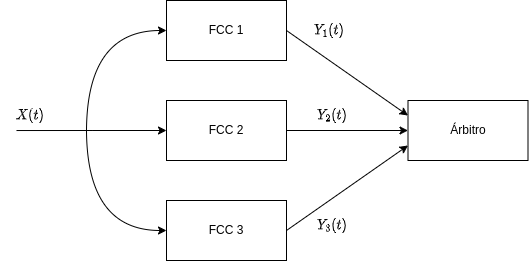
\includegraphics[width=\textwidth]{img/3_4_1_sincronizacion_1.png}
%         \caption{Computadoras de vuelo al inicio de la misión.}
%         \label{fig:3_4_1_sincronizacion_1}
%     \end{subfigure}
%     \begin{subfigure}[b]{0.49\textwidth}
%         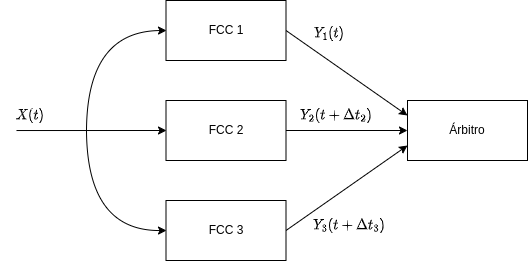
\includegraphics[width=\textwidth]{img/3_4_1_sincronizacion_2.png}
%         \caption{Al cabo de un período de tiempo, se desincronizarán.}
%         \label{fig:3_4_1_sincronizacion_2}
%     \end{subfigure}
%     \caption{A medida que transcurra el tiempo, la desincronización entre FCCs impactará en el sistema redundante.}
%     \label{fig:3_4_1_sincronizacion}
% \end{figure}

% Otra situación que puede presentarse, es que los resultados propuestos por las computadoras de vuelo $Y_1$, $Y_2$ e $Y_3$ correspondan a intervalos de tiempo distintos. Este caso es todavía peor que el anterior, ya que no se encuentra contemplado y el árbitro simplemente realizará la votación asumiendo que el dato es válido.

% \begin{figure}[htb]
%     \centering
%     \begin{subfigure}[b]{0.49\textwidth}
%         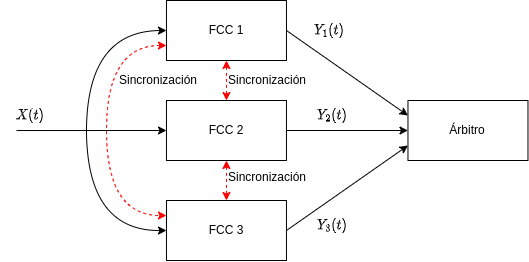
\includegraphics[width=\textwidth]{img/3_4_1_sincronizacion_3.png}
%         \caption{Las mismas computadoras de vuelo se encargan de la sincronización.}
%         \label{fig:3_4_1_sincronizacion_3}
%     \end{subfigure}
%     \begin{subfigure}[b]{0.49\textwidth}
%         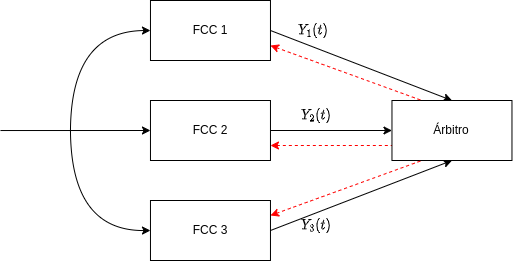
\includegraphics[width=\textwidth]{img/3_4_1_sincronizacion_4.png}
%         \caption{En este caso, la sincronización es administrada por el árbitro.}
%         \label{fig:3_4_1_sincronizacion_4}
%     \end{subfigure}
%     \caption{La sincronización entre nodos es necesaria para un correcto funcionamiento de las redundancias.}
% \end{figure}

% Se concluye que es mandatorio utilizar alguna técnica de sincronización entre los nodos. Como detalle de la figura \ref{fig:3_4_1_sincronizacion_3}, se muestra que la sincronización entre nodos presupone otro canal de comuniación más. Otra forma podría ser relegar la tarea de la sincronización al árbitro, aunque esto nuevamente presenta un punto singular de falla. Como se demostró en esta sección, el sincronismo es un aspecto crítico en el sistema redundante, por lo que se prefiere evitar esto último. Aunque de todas formas quisiera relegarse la sincronización al árbitro, este no solo recibirá mensajes de cada una de las FCCs, sino que además les enviará mensajes. Esto se muestra en la figura \ref{fig:3_4_1_sincronizacion_4}. Puede ocurrir una situación en la que el árbitro entregue valores distintos a cada una de las FCCs, evitando que estas se sincronicen.

Nuevamente, en los trabajos presentados en la sección \ref{sec:estado_del_arte}, la sincronización se ejecuta de manera periódica, donde las réplicas reajustan sus clocks. Para esto, cada una de ellas informa a las demás réplicas un valor asociado a su propio clock. Una vez que cada una conoce el estado de los clocks de todas las réplicas, estas buscan ponerse de acuerdo en un valor único. Si todas ellas poseen los mismos valores de entrada y ejecutan el mismo algoritmo, luego llegarán al mismo resultado.

En \cite{wensley1978sift} se presenta un trabajo del desarrollo de una computadora de vuelo con redundancias que utiliza un mecanismo de sincronización como el que se mencionó. Además, se analiza un caso particular, en el que una de las réplicas informa un valor distinto de su propio clock a las demás. Debido a que cada réplica tendrá información diferente acerca del estado del clock de esta réplica, luego no será posible lograr una sincronización. Esto genera la necesidad de que haya un consenso entre réplicas para los valores de clock, de manera que todas las réplicas lleguen al mismo resultado. Esto mismo puede ocurrir con otra información, como datos de sensores.

%Esta consiste en una comparación de valores asociados a los clocks de cada réplica. Cada una propone un valor distinto y estas buscarán ponerse de acuerdo en un valor único, el cual luego utilizarán como referencia para sincronizarse. Para que cada una de ellas llegue a la misma conclusión acerca del valor de clock correcto, si todas ellas ejecutan el mismo algoritmo y poseen los mismos valores de entrada, luego llegarán a la misma conclusión. En la figura \ref{fig:3_4_2_consenso_4} se muestra un caso en el que una de las computadoras de vuelo comparte valores de clock distintos a sus pares.

%\subsubsection{Consenso}\label{sec:consenso}
\subsubsection{Necesidad del Consenso entre Réplicas}\label{sec:consenso}
%\subsection{Consenso}\label{sec:consenso}

%Como se mostró en la figura \ref{fig:3_4_1_sincronizacion_3}, las computadoras de vuelo pueden comunicarse entre ellas para lograr una sincronización, por ejemplo compartiendo a sus pares un valor asociado a su propio clock interno. Cada FCC propone un valor distinto y estas buscarán ponerse de acuerdo en un valor único. Para que cada una de ellas llegue a la misma conclusión acerca del valor de clock correcto, si todas ellas ejecutan el mismo algoritmo y poseen los mismos valores de entrada, luego llegarán a la misma conclusión. En la figura \ref{fig:3_4_2_consenso_4} se muestra un caso en el que una de las computadoras de vuelo comparte valores de clock distintos a sus pares.

%La configuración de redundancia triple permite la tolerancia a fallas de 1 de las 3 réplicas. 
Si todas las réplicas sin fallas poseen los mismos valores de entrada y estas ejecutan el mismo algoritmo de votación, luego llegarán a la misma conclusión acerca de cuál es el valor correcto. Como fue mencionado en la sección anterior, esto es de especial importancia para llevar a cabo la sincronización. 

En las computadoras de vuelo de uso comercial, es común que se incorporen varios de los sensores dentro de la misma réplica. En estos casos, antes de ejecutar una estimación de la pose del vehículo, las réplicas deben primero obtener las mediciones de sus respectivos sensores y luego ponerse de acuerdo, es decir lograr un consesno, acerca de qué valor de sensor a utilizar para el cómputo. Lo que ocurre con los sensores es que estos sensan magnitudes físicas, por lo que entregarán magnitudes analógicas y siempre existirá una diferencia entre distintas réplicas, ya sea por diferencias propias de fabricación, por cuestiones de calibración, etc. Es por esto que se requiere lograr un consenso en un único valor. Otro escenario podría ser que cada una de las réplicas utilice las mediciones de sus propios sensores para obtener una estimación de la pose y que luego se ejecute una votación sobre este resultado, reduciendo la cantidad de intercambios de mensajes entre réplicas.

La configuración de triple redundancia, tal y como fue presentada hasta aquí, no resulta efectiva para estos casos donde cada réplica propone un valor y debe llegarse a un consenso. En la figura \ref{fig:TMR_sin_arbitro_consenso_falla} se muestra un ejemplo donde la réplica 1 informa un valor distinto a cada una de las demás. Este valor podría tratarse de valores de sensores o de resultados de la estimación de la pose. Lo que se observa es que este comportamiento genera que las réplicas 2 y 3 llegan a resultados distintos.

% \begin{figure}[htb]
%     \centering
%     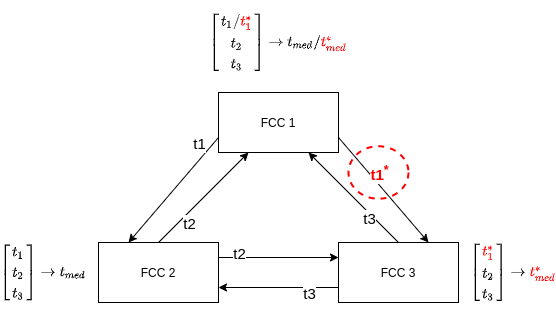
\includegraphics[width=0.6\textwidth]{img/3_4_2_consenso_4.png}
%     \caption{La FCC1 entrega un valor distinto de timing a las demás FCCs}.
%     \label{fig:3_4_2_consenso_4}
% \end{figure}

\begin{figure}[htb]
    \centering
    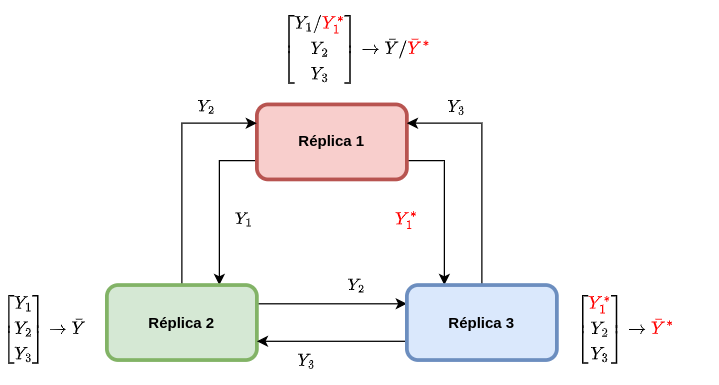
\includegraphics[width=0.8\textwidth]{img/TMR_sin_arbitro_consenso_falla.png}
    \caption{Las réplicas buscan ponerse de acuerdo en el valor correcto para la estimación de la pose. La réplica 1 manifiesta una falla e informa un valor diferente a cada una de las demás réplicas. Esto genera que las réplicas 2 y 3, las cuales no manifestaron ninguna falla, lleguen a resultados distintos, evitando así el consenso. En cuanto a la réplica 1, dependiendo de cuál haya sido realmente el valor que se haya calculado, esta obtendrá uno u otro resultado.}
    \label{fig:TMR_sin_arbitro_consenso_falla}
\end{figure}

%Una situación similar puede ocurrir con valores de entrada de sensores. En algunas computadoras de vuelo es común incorporar algunos sensores dentro de la misma réplica. En estos casos, antes de ejecutar una estimación de la pose del vehículo, las réplicas deben primero cada una obtener las mediciones de sus respectivos sensores y luego ponerse de acuerdo, es decir lograr un consesno, acerca de qué valor de sensor utilizar para el cómputo. Lo que ocurre con los sensores es que estos entregan mediciones analógicas, por lo que siempre existirá una diferencia entre distintas réplicas, ya sea por diferencias propias de fabricación, por cuestiones de calibración, etc.

%En este escenario, la FCC1 entrega dos valores distintos de su clock a las demás FCCs. Cada una de ellas luego realiza un promedio para llegar a un único valor. Lo que se observa es que las FCC2 y FCC3 calcularán un valor promedio distinto, es decir, no se sincronizarán.

Una posible solución podría ser realizar un nuevo intercambio con los valores obtenidos por cada réplica. Si bien esto sí permitiría lograr un consenso, el valor elegido estaría determinado por la réplica que presentó la falla, en este caso la réplica 1. Por otro lado, si esta nuevamente entrega un valor diferente a las réplicas 2 y 3, este nuevo intercambio tampoco servirá para lograr el consenso.

% Sin embargo, como se muestra en la figura \ref{fig:3_4_2_consenso_5}.

% \begin{figure}[htb]
%     \centering
%     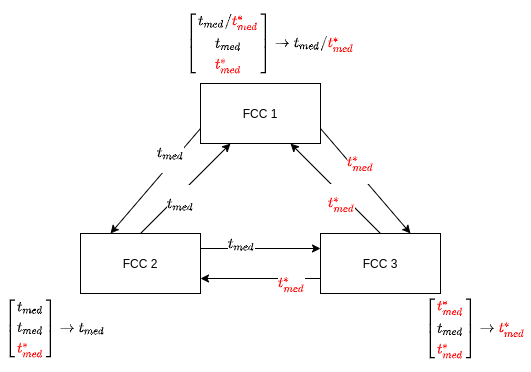
\includegraphics[width=0.6\textwidth]{img/3_4_2_consenso_5.png}
%     \caption{Luego de calcular los promedios, las FCCs intercambian sus resultados. Nuevamente, la FCC1 comete una falla en el envío del dato.}
%     \label{fig:3_4_2_consenso_5}
% \end{figure}

%Esta última situación, donde la FCC1 nuevamente comparte dos valores distintos a las demás, puede llevar a que las computadoras de vuelo no se sincronicen, algo que como ya se mencionó, es crítico para la correcta ejecución del algoritmo de tolerancia a fallas. Podría argumentarse que es demasiado pesimista pensar que la FCC1 puede producir la misma falla 2 veces de manera consecutiva, ya que existe una baja probabilidad de que ello suceda. Sin embargo, la situación planteada en esta sección puede tratarse como un tipo de falla de hardware que se manifiesta como comportamientos arbitrarios. Que exista una sincronización entre nodos redundantes implica que estos llegan a un consenso del paso del tiempo y el ritmo al que deben ejecutar sus tareas asignadas. Este consenso resulta crítico para que el sistema pueda detectar fallas correctamente.

%Algunos de los trabajos presentados anteriormente además realizan el algoritmo de votación sin la inclusión de un árbitro. Este caso es idéntico al de la figura \ref{fig:3_4_2_consenso_4}, es decir que el mismo problema del consenso también está presente para las votaciones acerca de resultados de cálculo de ley de control.

Este problema donde una réplica presenta información confusa se denomina \textit{The Byzantine Generals Problem} y se analiza en \cite{lamport2019byzantine}. Este demuestra que se requieren $3 m + 1$ réplicas para tolerar $m$ que manifiesten este tipo de fallas. Otros de los trabajos que analizan este mismo problema son \cite{pease1980reaching} y \cite{wensley1978sift}. En este último se presenta el diseño de una computadora de vuelo tolerante a fallas que utiliza los resultados del \textit{Byzantine Generals Problem} para alcanzar la sincronización.

%El modelo de falla que se está considerando representa un comportamiento anómalo arbitrario, es decir, que a priori no se asume nada acerca de la falla. A este tipo de comportamiento se lo denomina falla bizantina o \textit{Byzantine Fault} en inglés y básicamente consiste en asumir que el elemento que manifiesta la falla presenta un comportamiento arbitrario. Por ejemplo, un sensor puede dejar de funcionar repentinamente y no dar más respuesta, puede dejar de enviar respuesta por un período de tiempo y luego volver a funcionar, podría también enviar datos a un microcontrolador pero que esos datos sean incoherentes, etc. El modelo de falla bizantina no asume modos de falla, sino que el comportamiento es arbitrario \cite{roth2021not}\cite{hiergeist2017internal}\cite{lala1994architectural}. El nombre proviene de un problema denominado \textit{The Byzantine Generals Problem}, formalizado en \cite{lamport2019byzantine}. Otros trabajos que tratan el mismo problema son \cite{pease1980reaching} y \cite{wensley1978sift}. Este último, presenta el diseño de una computadora de vuelo tolerante a fallas que utiliza los resultados del \textit{Byzantine Generals Problem} para realizar distintas tareas de redundancia.\\

%Una forma de alivianar esta tarea es la de considerar un modelo de falla de hardware más conservador, donde se asume que una falla de hardware consiste en que esta presente un comportamiento anómalo arbitrario, es decir, de cualquier tipo. A este tipo de comportamiento se lo denomina falla bizantina o \textit{Byzantine Fault} en inglés y básicamente consiste en asumir que el elemento que manifiesta la falla presenta un comportamiento arbitrario. Por ejemplo, un sensor puede dejar de funcionar repentinamente y no dar más respuesta, puede dejar de enviar respuesta por un período de tiempo y luego volver a funcionar, podría también enviar datos a un microcontrolador pero que esos datos sean incoherentes, etc. El modelo de falla bizantina no asume modos de falla, sino que el comportamiento es arbitrario \cite{roth2021not}\cite{hiergeist2017internal}\cite{lala1994architectural}. Se define un sistema tolerante a este tipo de fallas.

En la figura \ref{fig:byzantine_ejemplo_3} se muestra un caso donde la réplica 1 entrega el mismo valor a las réplicas 2 y 4, pero entrega un valor diferente a la 3. A partir de un nuevo intercambio entre las réplicas 2, 3 y 4 puede llegarse a un consenso acerca de un úncio valor correspondiente a la réplica 1. En este caso al tener 3 réplicas que no manifiestan este tipo de fallas, puede hacerse una votación 2 de 3 sin involucrar a la réplica con fallas, es decir a la 1.


%Se plantea una situación como la de la figura \ref{fig:3_4_2_consenso_4}, pero en este caso se utilizan 4 computadoras de vuelo en lugar de 3. En este caso, las computadoras de vuelo deben sincronizarse. Para lograrlo, ellas comparten un valor de timestamp, que pueden utilizar para ajustar sus clocks. En la figura \ref{fig:Byzantine_Generals_Problem_5} se muestra un escenario en el que una de las computadoras de vuelo presenta una falla tal que le informa un valor distinto a cada una de sus pares.

% \begin{figure}[htb]
%     \centering
%     \begin{subfigure}[b]{0.4\textwidth}
%         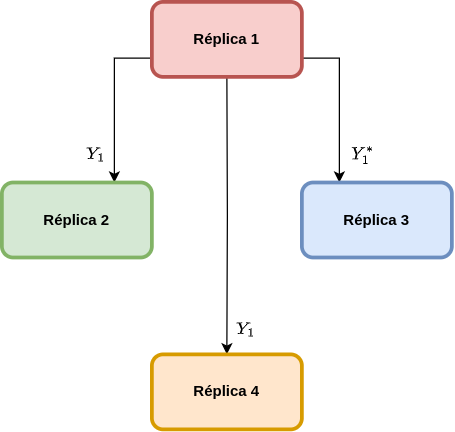
\includegraphics[width=\textwidth]{img/byzantine_ejemplo_1.png}
%         \caption{Intercambio 1.}
%         \label{fig:byzantine_ejemplo_1}
%     \end{subfigure}\hfill
%     \begin{subfigure}[b]{0.55\textwidth}
%         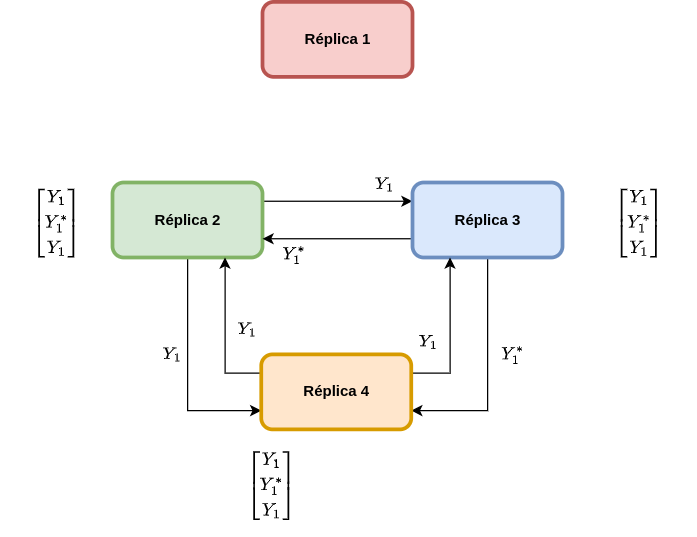
\includegraphics[width=\textwidth]{img/byzantine_ejemplo_2.png}
%         \caption{Intercambio 2.}
%         \label{fig:byzantine_ejemplo_2}
%     \end{subfigure}
%     \caption{Debido a la existencia del bus, las FCCs no pueden mentir acerca de su \textit{timestamp}. Luego, todas llegan a un consenso de manera casi trivial.}
%     \label{}
% \end{figure}

\begin{figure}[htb]
    \centering
    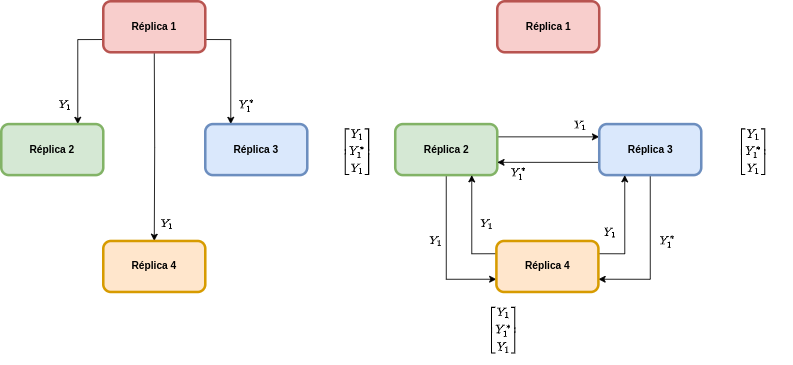
\includegraphics[width=\textwidth]{img/byzantine_ejemplo_3.png}
    \caption{En la primera imagen se muestra que debido a una falla la réplica 1 le entrega un valor distinto a la réplica 3. A partir de un segundo intercambio entre las réplicas sin fallas, puede llegarse a un consenso acerca del valor indicado por la réplica 1.}
    \label{fig:byzantine_ejemplo_3}
\end{figure}

% \begin{figure}[htb]
%     \centering
%     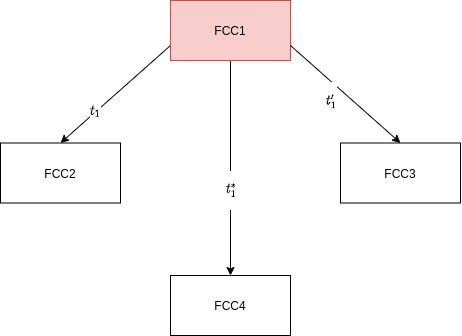
\includegraphics[width=0.5\textwidth]{img/Byzantine_Generals_Problem_5.png}
%     \caption{Debido a una falla, la computadora de vuelo 1 le entrega valores distintos de timestamp a las demás.}
%     \label{fig:Byzantine_Generals_Problem_5}
% \end{figure}

% \begin{figure}[htb]
%     \centering
%     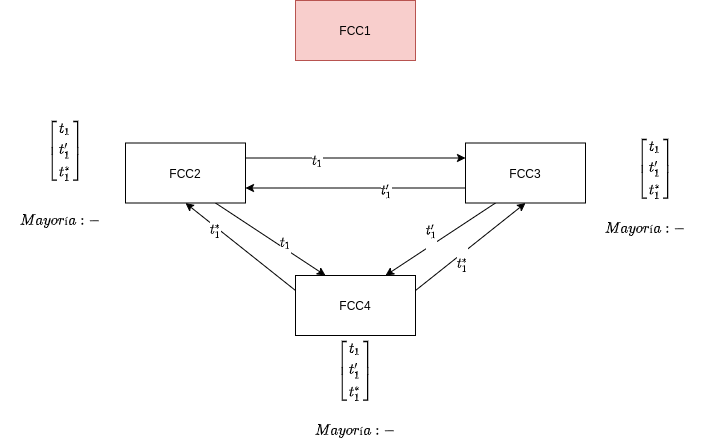
\includegraphics[width=0.7\textwidth]{img/Byzantine_Generals_Problem_6.png}
%     \caption{Las FCC2, 3 y 4 comparten entre sí lo que les dijo la FCC1 a cada una y llegan a la conclusión de que la información es inconsistente.}
%     \label{fig:Byzantine_Generals_Problem_6}
% \end{figure}

Esta configuración también permite tolerar el caso en el que la réplica 1 entrega un valor diferente a cada una de las otras 3 réplicas. En ese caso, cuando se ejecute el segundo intercambio, al detectar que todos los valores son diferentes, simplemente se ignorará a la réplica 1. Esto podría ser por ejemplo asumiendo algún valor por defecto.

%A través de un segundo intercambio, las FCC 2, 3 y 4 llegan a la conclusión de que el timestamp de la FCC1 no es claro. En este caso, descartan el valor. Luego de hacer todos los intercambios de timestamp, las FCCs podrán aplicar internamente la sincronización, por ejemplo, calculando un promedio de todos los timestamp. \textbf{Dado que todas las FCCs tendrán la misma información de timestamp entregado por las demás FCCs, luego todas llegarán al mismo promedio y se sincronizarán}.\\

%Un aspecto interesante es el hecho de que en el paper original, se hace una analogía entre un nodo redundante con fallas y un nodo traidor, es decir, que busca corromper el consenso de los demás nodos. Esto lo que quiere decir es que las fallas presentadas por las computadoras de vuelo pueden ser justamente de cualquier característica, incluso al extremo de presentar un comportamiento malicioso, con el objetivo de perjudicar al sistema \cite{lala1994architectural}. Esto sienta las bases para la tolerancia a fallas de hardware arbitrarias.\\

%La implementación del algoritmo tolerante a fallas arbitrarias resulta costoso. Para poder tolerar fallas provenientes de 1 FCC se requiere un total de 4 computadoras de vuelo. Además, debe haber una interconexión entre las 4 computadoras y ellas deben intercambiar información continuamente para poder detectar y enmascarar la falla. A todo esto se le debe sumar, la necesidad de la sincronización.\\

Sin dudas el hecho de utilizar 4 réplicas para tolerar solamente la falla de 1 de ellas encarece mucho el sistema. Además, debe haber una interconexión entre las 4 y estas deben realizar 2 intercambios de información por cada nuevo resultado calculado.

Una de las cuestiones que no se menciona en el problema original, es el caso en el que las réplicas constituyen sistemas de tiempo real, algo que sí ocurre con las computadoras de vuelo. Otro de los puntos que caracterizan al problema original, es el hecho de que la comunicación entre las réplicas es 1 a 1. Si el sistema tiene la características de funcionar de manera sincronizada e implementar una comunicación a través de un bus, luego el problema del consenso puede resolverse de una manera más simple.

%\subsection{Requerimientos Comunes en Sistemas con Redundancias}

%Todos los trabajos y ejemplos presentados en la sección anterior comparten la característica de implementar la tolerancia a fallas utilizando varias copias del mismo elemento de hardware. Estas copias trabajan en paralelo y se comparan los resultados obtenidos por cada una de ellas. Las fallas se detectan cuando ocurre una diferencia en los resultados de las copias.\\

%{\color{red} EXPLICAR Y JUSTIFICAR EL POR QUÉ DE LAS REDUNDANCIAS POR SOBRE EL USO DE COMPONENTES DE ALTÍSIMA CALIDAD, EN UN PÁRRAFO.}

%A continuación, se describen algunas de las características detectadas.

\subsection{Simplificación del Problema}

%Una de las cuestiones que no se menciona en el problema original, es el caso en el que los nodos constituyen sistemas de tiempo real. Las computadoras de vuelo deben realizar tareas que requieren determinismo temporal, por ejemplo cálculo de la ley de control, estimación de la pose, etc... En el problema original, los nodos pueden enviar sus mensajes a sus pares en cualquier momento y en cualquier orden. Otro de los puntos que caracterizan al problema original, es el hecho de que la comunicación entre los nodos es 1 a 1. Debido a esto, los traidores pueden entregar información confusa a sus pares para tratar de romper el consenso. Esto es lo que vuelve complejo al problema \cite{lamport2019byzantine} y costosa a su solución \cite{roth2021not}. Si el sistema en cuestión presenta la características de ser de tiempo real e implementar una comunicación a través de un bus, en conjunto, luego el problema del consenso puede simplificarse mucho.\\

Como se pudo ver en la sección \ref{sec:estado_del_arte}, varios de los trabajos utilizan un bus para la comunicación entre las réplicas. Esto se presenta tanto en el caso del avión como en varios de los ejemplos de UAVs. También se mostró que una de las computadoras de vuelo comerciales, la de la empresa Embention, utiliza el bus CAN para resolver las comunicaciones entre réplicas con el árbitro. %Esto tambień ocurre por ejemplo en los automóviles, los nodos que se encuentran repartidos por todo el vehículo se comunican a través de redes como CAN\cite{specification1991bosch} o FlexRay\cite{nxpAN12233}. Todos los nodos de la red se encuentran conectados al mismo bus de comunicación, por lo que cuando un nodo envía un mensaje a través del bus, todos los demás nodos reciben el mismo mensaje.
Esto presenta una diferencia con lo planteado en la sección anterior, ya que la existencia de un bus automáticamente elimina la posibilidad de que una de las réplicas pueda entrgar información diferente a sus pares. Puede compararse la figura \ref{fig:TMR_sin_arbitro_consenso_falla} con la figura \ref{fig:TMR_bus}. Siempre que alguna de las réplicas envíe un mensaje a través del bus, este será recibido por todas las demás.

%En sistemas de tiempo real para aplicaciones \textit{safety-critical}, es común encontrar sistemas distribuidos con comunicación a través de un bus. Esto se mencionó en la sección \ref{sec:estado_del_arte} tanto para el caso del avión como para varios de los ejemplos de UAVs presentados. Esto tambień ocurre por ejemplo en los automóviles, los nodos que se encuentran repartidos por todo el vehículo se comunican a través de redes como CAN\cite{specification1991bosch} o FlexRay\cite{nxpAN12233}. Todos los nodos de la red se encuentran conectados al mismo bus de comunicación, por lo que cuando un nodo envía un mensaje a través del bus, todos los demás nodos reciben el mismo mensaje.

% \begin{figure}[htb]
%     \centering
%     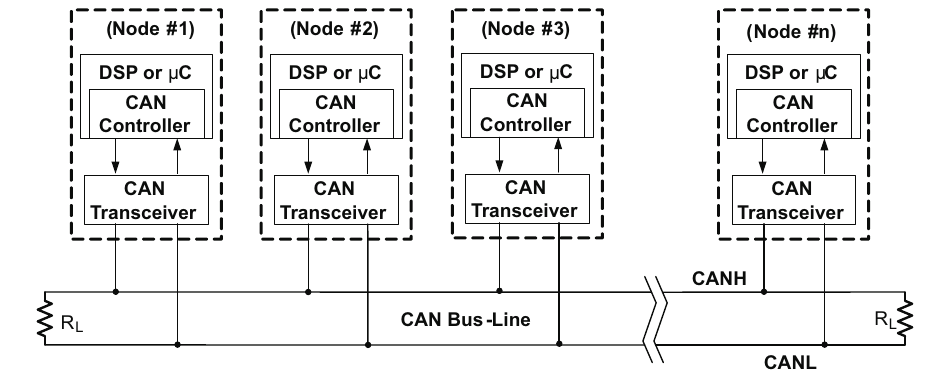
\includegraphics[width=\textwidth]{img/red_CAN.png}
%     \caption{Todos los nodos se encuentran conectados al mismo bus de comunicaciones. En el caso del bus CAN, se compone de dos cables, CAN-H y CAN-L, terminados en sus extremos por resistencias de adaptación. La imagen se extrajo de \cite{texasSLOA101B}.}
%     \label{fig:red_CAN}
% \end{figure}

%Esto presenta una diferencia respecto de lo planteado en \textit{The Byzantine Generals Problem}, ya que la existencia de un bus común a todos los nodos automáticamente elimina la posibilidad de que uno de los miembros de la red pueda enviar información diferente a sus pares. Puede compararse la figura \ref{fig:byzantine_bus_1} con la figura \ref{fig:Byzantine_Generals_Problem_5}.

\begin{figure}[htb]
    \centering
    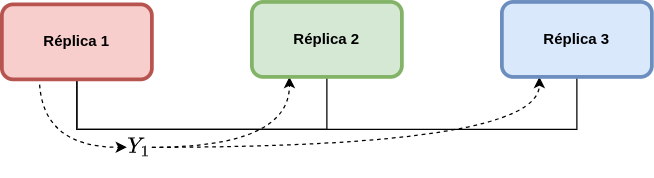
\includegraphics[width=0.8\textwidth]{img/TMR_bus.png}
    \caption{La conexión tipo bus obliga a que la información enviada por cada réplica sea recibida por todas las demas, evitando el envío de información confusa. El mismo valor $Y_1$ será recibido por las réplicas 2 y 3.}
    \label{fig:TMR_bus}    
\end{figure}

% \begin{figure}[htb]
%     \centering
%     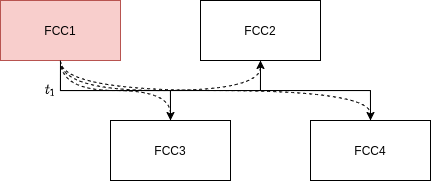
\includegraphics[width=0.6\textwidth]{img/byzantine_bus_1.png}
%     \caption{En este caso, la conexión tipo bus no permite el envío de información diferente a los demás miembros. La FCC1 envía el valor $t_1$ y todos sus pares reciben el mismo valor.}
%     \label{fig:byzantine_bus_1}    
% \end{figure}

Si bien el uso de un bus de comunicaciones simplifica el problema del consenso, existen otras cuestiones que deben tenerse en cuenta. Uno de los factores importantes es el hecho de que en esta configuración el bus se vuelve un punto singular de fallas, ya que todas las comunicaciones pasan por este. Para solucionar esto puede utilizarse más de un bus en paralelo, asumiendo que solo uno de ellos podrá fracasar en su funcionamiento al mismo tiempo \cite[p.~157]{kopetz-2011}. Esto es algo que también se pudo ver en los ejemplos de la sección \ref{sec:estado_del_arte}, como en el caso del avión.

Teniendo en cuenta la necesidad del sincronismo entre las réplicas explicado en la sección \ref{sec:necesidad_del_sincronismo}, la posibilidad de que ocurran colisiones es un problema que puede perjudicar el funcionamiento del mecanismo de tolerancia a fallas. Una colisión puede causar que la información nunca llegue a su destino o bien que llegue con un retraso, por ejemplo si se utiliza un mecanismo de retransmisión para asegurar el envío del mensaje.

La manera de solucionar esto es forzando a que las réplicas deban tomar turnos para enviar un mensaje por el bus. Para lograr este comportamiento, cada una de estas debe saber en qué momentos puede utilizar el bus de comunicaciones para enviar un mensaje y cuándo no. Una vez más, este comportamiento también se encuentra presente en varios de los trabajos presentados en la sección \ref{sec:estado_del_arte}, incluido el ejemplo del avión, mediante el uso de un acceso al medio TDMA.

%Esto puede lograrse si las réplicas trabajan de manera sincronizada, algo que ya de por sí es necesario.


%estos deben tomar turnos para enviar la información a sus pares. De otra forma, habría una colisión en el bus, lo que puede causar que la información nunca llegue a su destino o que llegue con un retraso, por ejemplo si se utiliza un mecanismo de retransmisión para asegurar el envío del mensaje.

%Como contrapartida, debido a que los nodos comparten canal de comunicación, estos deben tomar turnos para enviar la información a sus pares. De otra forma, habría una colisión en el bus y la información nunca llegaría a su destino. Sumado a esto, el bus se convierte en un punto singular de falla, ya que es posible que un problema en el bus deje a los nodos incomunicados.\\

%\subsubsection{Consenso}

%Al igual que como se hizo en la sección \ref{sec:consenso}, se analiza el problema del consenso utilizando un bus. El ejemplo que se presentó anteriormente fue el necesario para lograr una sincronización entre las FCCs y se mostró que el enviar información distinta a cada computadora de vuelo puede romper el sincronismo muy fácilmente.\\

% Como ya se mencionó, las FCCs deben tomar turnos para utilizar el medio físico. En las próximas secciones se explicará cómo se puede lograr esto, aquí se asume que las FCCs respetan sus turnos para utilizar el medio físico compartido. En la figura \ref{fig:byzantine_bus_2}, la FCC1 accede al medio y envía su valor de timestamp. Las demás FCCs reciben el mismo valor, por estar conectadas al mismo bus de comunicación. Luego, las FCC2 y 3 repiten esto mismo. En la figura \ref{fig:byzantine_bus_3} se muestra que todas tienen la misma información respecto de sus pares. Luego por ejemplo, si calculan un promedio, llegarán al mismo resultado y se sincronizarán correctamente.

% \begin{figure}[htb]
%     \centering
%     \begin{subfigure}[b]{0.34\textwidth}
%         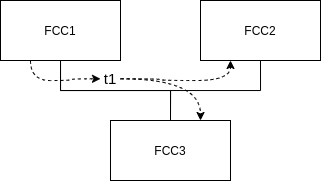
\includegraphics[width=\textwidth]{img/byzantine_bus_2.png}
%         \caption{La FCC1 envía su \textit{timestamp} hacia las demás.}
%         \label{fig:byzantine_bus_2}
%     \end{subfigure}\hfill
%     \begin{subfigure}[b]{0.49\textwidth}
%         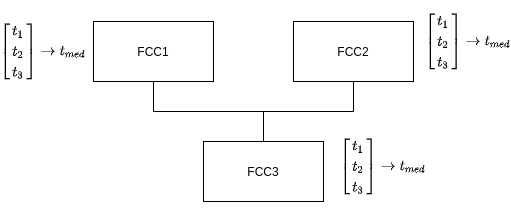
\includegraphics[width=\textwidth]{img/byzantine_bus_3.png}
%         \caption{Luego de finalizar los intercambios, todas las FCCs llegan al mismo resultado de \textit{timestamp} para sincronizarse.}
%         \label{fig:byzantine_bus_3}
%     \end{subfigure}
%     \caption{Debido a la existencia del bus, las FCCs no pueden mentir acerca de su \textit{timestamp}. Luego, todas llegan a un consenso de manera casi trivial.}
%     \label{}
% \end{figure}

A partir de este análisis, se puede ver que para el caso de un sistema de tiempo real con un bus de comunicaciones y donde las réplicas funcionan de manera sincronizada, el problema del consenso es más sencillo, ya que no se requiere el uso de 4 réplicas ni tampoco es necesario realizar tantos intercambios de mensajes. 
%que lo que se muestra en \textit{The Byzantine Generals Problem}. De todas maneras, lo que se presenta aquí es un primer análisis, ya que se ha asumido que no hay colisiones en el bus y que los nodos se encuentran sincronizados. 
De esta manera la configuración de triple redundancia donde las réplicas funcionan de manera sincronizada, implementan una comunicación a través de un bus de comunicaciones y respetan sus turnos para enviar mensajes, permite implementar mecanismos para tolerar una falla simultánea de 1 de las 3 réplicas.


%donde Se concluye que, para que la computadora de vuelo pueda implementar distintos mecanismos de tolerancia a fallas, esta debe contar con una interfaz que le permita la comunicación a través de un bus de comunicaciones.

%\subsection{Uso de Componentes COTS}

%\textbf{{\color{red} COMPLETAR}}

